%%%%%%%%%%%%%%%%%%%%%%%%%%%%%%%%%%%%%%%%%
% Revista Difu100cia
%%%%%%%%%%%%%%%%%%%%%%%%%%%%%%%%%%%%%%%%%
\documentclass[12pt]{difu100cia} % clase difu100cia

%----------------------------------------------------------------------------------------
%	PAQUETES ADICIONALES
%----------------------------------------------------------------------------------------



%----------------------------------------------------------------------------------------
%	DECLARACION DE COMANDOS
%----------------------------------------------------------------------------------------




%----------------------------------------------------------------------------------------
%	INFORMACION DEL ARTICULO
%----------------------------------------------------------------------------------------

\title{Acciones que promueven la inclusión del marketing digital en MIPYMES de Xicotepec} % Titulo del articulo en ingles
% Autores
\author[1]{\authorstyle{Quiroz Ramírez-Isabel}}
\author[1]{\authorstyle{Cruz Suárez- Silvia Denisse}\thanks{Autor de correspondencia}}
\author[1]{\authorstyle{Galindo González-Oscar}}
\author[1]{\authorstyle{Amador Mendoza- Evelin1}}
\author[1]{\authorstyle{Velázquez Vargas-José Rubén}}
\author[1]{\authorstyle{Tolentino Castillo- Guadalupe}}
%\author[2]{\authorstyle{Juán Perez}}
\affil[1]{\institution{Universidad Tecnológica de Xicotepec de Juárez (UTXJ), Área Económico-Administrativa, \authorcr Cuerpo Académico. Desarrollo empresarial, \authorcr Av. Universidad Tecnológica No. 1000, Col. Tierra Negra, Xicotepec de Juárez, Puebla. C.P. 73080. \authorcr quirozisabel1983@hotmail.com,\{(isabel.quiroz, silvia.cruz, oscar.galindog, evelin.amador, ruben.velazquez, guadalupe.tolentino\}@utxicotepec.edu.mx }}
%\affil[2]{\institution{Universidad Tecnológica de Xicotepec de Juárez}}

%----------------------------------------------------------------------------------------
%   Fecha de publicación
%----------------------------------------------------------------------------------------

\publishrange{Mayo - Agosto 2022}
\volume{13}
\num{2}
\published{12 de agosto de 2022}

%----------------------------------------------------------------------------------------

\begin{document}

\selectlanguage{spanish} % selecciona espanol como idioma
%\selectlanguage{english} % Selecciona ingles como idioma
\thispagestyle{firstpage} % Aplica el estilo en la primera pagina sin cabeceras y pie de pagina
\maketitle % Imprime el titulo
\pagestyle{fancy}

%----------------------------------------------------------------------------------------
%	RESUMEN
%----------------------------------------------------------------------------------------

\begin{abstract}[english]
This research work aims to analyze the different activities that allow the implementation of digital marketing in MSMEs in Xicotepec. It is vital for companies in general to develop strategies that strengthen their capacity and the continuous search for competitive advantages, making it essential to research and implement improvements in all areas. 
As a proposal on this occasion, we present research that aims to articulate different mechanisms that allow MSMEs in Xicotepec the knowledge, management, and inclusion of digital marketing in their operations since because of the pandemic situation we are going through, was caused these introduced in an untimely manner the sale of their products and services with the use of digital tools; using mainly WhatsApp and Facebook, as means of advertising and distribution channel for their products, while some others implemented only the home service.
Derived from the above, a solid economic recession was generated in Xicotepec. It is now essential to identify, define and implement different strategies that allow the economic momentum in the region to contribute to the survival and promotion of MSMEs with the help of digital marketing.
For all the above described, the importance of this research is justified by pointing to the use of digital marketing to contribute to the economic recovery of MSMEs in Xicotepec de Juárez, which according to data from the 2019 Economic Census, the sectors that concentrated the most significant number of economic units were: retail trade (1,880 units), manufacturing industries (639 units) and other services except government activities (617 units).

\end{abstract}

\keywords[english]{ Digital marketing, MSMEs, digital tools}

\begin{abstract}[spanish]
El presente trabajo de investigación tiene como finalidad analizar las diferentes actividades que permitan la implementación del marketing digital en las MIPYMES de Xicotepec. Es de vital importancia para las empresas en general el desarrollo de estrategias que promuevan el fortalecimiento de su capacidad y la búsqueda continua de ventajas competitivas, mismas que hacen primordial la investigación e implementación de mejoras en todas las áreas. 
Como propuesta se presenta esta investigación que apunta a la articulación de diferentes mecanismos que permitan a las MIPYMES de Xicotepec adquirir el conocimiento, manejo e inclusión del marketing digital en sus operaciones, ya que a consecuencia de la pandemia generada por el virus COVID 19 que estamos atravesando, se ocasiono que estas entidades económicas introdujeran de manera intempestiva la venta de sus productos y servicios con la utilización de herramientas digitales; utilizando principalmente WhatsApp y Facebook, como medios de publicidad y canal de distribución para sus productos, mientras que algunos otros implementaron solo el servicio a domicilio.
Derivado de lo anterior se generó una fuerte contracción económica en Xicotepec por lo que es primordial  identificar, definir y aplicar diferentes estrategias que permitan el impulso económico en la región coadyuvando a la supervivencia e impulso de las MIPYMES, mediante la ayuda del marketing digital.
Por todo lo anteriormente descrito, se justifica la relevancia de esta investigación apuntando a la utilización del marketing digital para contribuir a la recuperación económica de las MIPYMES de Xicotepec de Juárez, Puebla; que según los datos del Censo Económico 2019, los sectores que concentraron mayor cantidad de unidades económicas fueron: comercio al por menor (1,880 unidades), industrias manufactureras (639 unidades) y otros servicios exceptuando actividades gubernamentales (617 unidades).
\end{abstract}

\keywords[spanish]{Marketing digital, MIPYMES, herramientas digitales}

%----------------------------------------------------------------------------------------
%	ARTICULO
%----------------------------------------------------------------------------------------

\section{Introducción}
Es importante definir que como estrategia central objeto de esta investigación se abordará principalmente el marketing digital, mismo que se ha convertido en una herramienta para el comercio.
Según datos del INEGI el 99.8% de las unidades de negocio, pertenecen al segmento de micro, pequeña y mediana empresa, con más de 4.1 millones de empresas que aportan el 42% del Producto Interno Bruto. (PIB).
En el año 2020 más de un millón de empresas tuvieron que cerrar sus puertas. Cabe mencionar que durante este período también se establecieron 619,443 nuevas empresas.
El 30 de enero del 2020, la Organización Mundial de la Salud (OMS), marcó el inicio de una emergencia de salud pública de preocupación internacional, considerada ahora pandemia, ocasionada por el incremento de casos causados por el virus COVID-19, cuyos contagios se extendieron en varios países del mundo.
Es menester de este trabajo; presentar los resultados del estudio realizado y poder a través de ellos proponer las líneas de acción a seguir para la adquisición e implementación de mecanismos necesarios que permitirán a resumidas cuentas, el posicionamiento de la actividad económica de las MIPYMES: y que al mismo tiempo generará la reactivación económica de Xicotepec de Juárez, Puebla; minimizando así los efectos de la Pandemia causada por el virus SARS COV 2.


\section{Marco teórico}

Al hablar de marketing podemos encontrar diferentes definiciones, por ejemplo: Philip Kotler la define como “un proceso social y administrativo mediante el cual grupos e individuos obtienen lo que necesitan y desean a través de generar, ofrecer e intercambiar productos de valor con sus semejantes” .
Por otra parte, para Stanton, Et. al, indican que: "El marketing es un sistema total de actividades de negocios ideado para planear productos satisfactores de necesidades, asignarles precios, promover y distribuirlos a los mercados meta, a fin de lograr los objetivos de la organización".
Según el libro de la Guerra del marketing, para John A. Howard, de la Universidad de Columbia, "el marketing es el proceso de: 1) Identificar las necesidades del consumidor, 2) conceptualizar tales necesidades en función de la capacidad de la empresa para producir, 3) comunicar dicha conceptualización a quienes tienen la capacidad de toma de decisiones en la empresa. 4) conceptualizar la producción obtenida en función de las necesidades previamente identificadas del consumidor y 5) comunicar dicha conceptualización al consumidor".
De las contribuciones más importantes que ha realizado Kotler es la ampliación del concepto de marketing, estableciendo que es una nueva forma de comunicación e intercambio con los clientes, no solo para comercializar sino también para forjar experiencias únicas. Es decir, que el marketing puede utilizarse para influenciar el comportamiento de diversos sectores de la población al ser un proceso social y administrativo. De esta manera, los consumidores obtienen lo que desean a través de ofertas e intercambios de productos de valor y como vendedor creas un lazo de fidelidad con éstos.  
El marketing a través del tiempo ha evolucionado dando como resultado varias transformaciones en pro de la forma de vender los productos y servicios de las empresas, posicionamiento de las marcas, fidelización de los clientes y actualmente hacer llegar más rápido esta información de las empresas a sus clientes reales y potenciales en satisfacción de las necesidades de estos últimos.
El marketing digital se desarrolla en cuatro eras las cuales son:
Marketing 1.0: Es el marketing que la mayoría de las empresas realiza y cuya primicia era enfocarse en la inversión para el desarrollo del producto. 
Marketing 2.0: A diferencia del anterior, este tipo de marketing ya no solo busca vender calidad, sino que además comienzan a entender las necesidades y hábitos de sus clientes, con el objetivo de crear nuevos productos y servicios basándose en sus comportamientos, pues ahora es el consumidor quien define el valor del producto. 
Marketing 3.0: Se basa completamente en comprender y conocer al cliente más allá de querer venderles un producto o servicio. En este estado las empresas se diferencian entre sí por sus valores. 
Marketing 4.0: La cuarta etapa del marketing hace hincapié a la era digital y la interconectividad con las nuevas tecnologías que actualmente son de suma importancia para los mercadólogos y la sociedad. Por lo que, es una transición de lo tradicional a lo digital. A su vez, establece nuevas métricas para llegar más rápido a nuevos mercados. Su objetivo es la confianza y fidelización del cliente (Cousillas, 2018).
Gracias a Tim Berner-Lee, creador del sistema de transmisión de datos que se extendió de manera mundial y lo bautizó como la “Word Wide Web”  (Velazco, 2015), el día de hoy millones de usuarios pueden crear sitios que les pueden abrir puertas y aprovechar los espacios para hacer llegar su mensaje más allá del alcance que ofrecen los medios tradicionales. 
El marketing digital es una nueva forma comercial que lleva a cabo la empresa, utilizando la telemática y que permite a sus clientes o clientes potenciales conseguir: efectuar una consulta de un producto y/o seleccionar o adquirir la oferta existente en un momento, de un determinado producto. 
Hoy en día gracias a las redes sociales como Facebook, Twitter, tiktok, entre otros, los comerciantes pueden hacer llegar su publicidad de una manera más fácil, rápida, económica, y sobre todo teniendo el dominio de la información que proporcionan a sus clientes, contando con la ventaja adicional de poder contactarse con sus posibles clientes sin la necesidad de estar en el mismo espacio físico. 
Por lo anterior entenderemos al marketing digital como: los procesos y gestiones necesarias para conocer las necesidades del cliente, transformándolas en conceptos de servicios o productos que ofrecen las empresas a sus consumidores potenciales a través de la difusión de los conceptos de servicios o productos mediante los diferentes medios digitales existentes. Es por ello que se hace de primordial importancia implementar algunas acciones que coadyuven a que las MIPYMES de Xicotepec de Juárez, Puebla; hagan uso correcto del marketing digital para el incremento de su competitividad.

\section{Descripción del modelo}
El modelo que se utiliza para la presente investigación es de tipo cuantitativo, el cual permitirá recolectar datos basados en la opinión de empresarios sobre la implementación del uso del marketing digital y posteriormente será procesada en valores numéricos para la toma de decisiones. 

Respecto al instrumento será aplicado en la zona principal de Xicotepec, con la finalidad de identificar y definir acciones que permitan el impulso económico de las MIPYMES, a través de la inclusión del marketing digital.

Respecto a la identificación de empresas que fueron parte del muestreo, se utilizó la base de datos obtenida en el DENUE (Directorio Estadístico Nacional de Unidades Económicas), que depende del Instituto Nacional de Estadística y Geografía (INEGI). Señalando que se utilizó una clasificación de empresas a las que se les censó, entre ellas fueron dedicadas a: servicios al por mayor, comercio al por menor, servicios de esparcimiento, culturales, deportivos y otros servicios de alojamiento temporal, así como de preparación de alimentos y bebidas.      
\end{figure}

\section{Descripción de la metodología}
Primera parte:

1.- Preliminares
•	Cómo primera actividad se diseñó un instrumento de recolección de datos, mediante un formulario de google forms, el cual contempló 12 reactivos entre los cuales se cuestionó si las micro, pequeñas y medianas empresas utilizan medios electrónicos o algunas apps para dar a conocer sus productos y servicios, así como si el promocionarse en redes sociales ha aumentado las ventas de sus productos en estos últimos periodos, cabe señalar que dicho cuestionario fue aplicado a una muestra representativa de 339 empresas, resultado de una población de 2,858 empresas registradas en DENUE 2022, como se muestra en la figura 1, utilizando un nivel de confianza del 95%.

\begin{figure}[!ht]
	\centering
	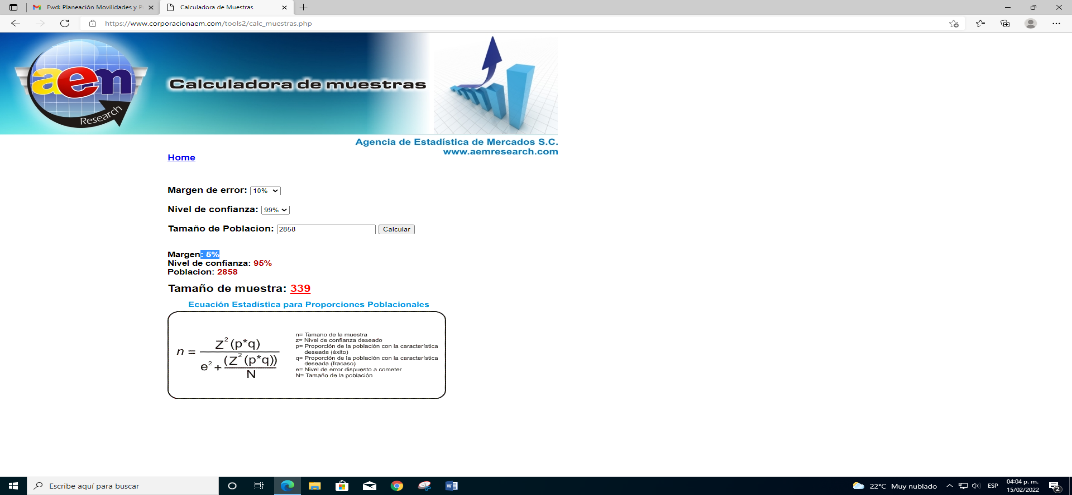
\includegraphics[width=\linewidth]{Figura 1.png}
	\caption{Muestra representativa del censo}
	\label{diagrama_estructura_rfnoc}
\begin{enumerate}
  \item El IP del FPGA, donde se concentra la mayor parte del trabajo realizado, puede ser escrita en Verilog, VHDL, o integrar un IP de Xilinx, con la única condición de que use el protocolo AXI Stream. Se deben de considerar las señales de entrada - salida previamente establecidas y el uso de los registros.  
  \item El control del bloque representa la lógica digital en el lado del software, declara el flujo de datos entrada - salida, y declara las propiedades reconfigurables del bloque de procesamiento de señales por medio de un archivo XML.  
  \item La integración a GNU Radio se logra agregando los bloques RFNoC como un modulo OOT.  la programación de los archivos de enlace es muy similar a la de GNU Radio.  
\end{enumerate}

\begin{figure}[!htb]
	\centering
	\includegraphics[width=\linewidth]{Diagra_rfnoc.png}
	\caption{Componentes para el desarrollo de un bloque RFNoC.}
	\label{diagrama_bloque_rfnoc}
\end{figure}

\subsection{USRP X300}

Ettus Research USRP X300 es una plataforma de SDR de alto rendimiento para diseñar e implementar sistemas de comunicación inalámbricas de próxima generación, este cuenta con las siguientes características \cite{ettusresearch}:

\begin{itemize}
    \item Dos ranuras para las tarjetas hijas de RF de banda ancha con las siguientes características:
    \begin{itemize}
        \item Hasta 160 MHz de ancho de banda por cada una. 
        \item Cubre desde CD (corriente directa) hasta 6 GHz. 
    \end{itemize}
    \item Consta de un FPGA Kintex-7 de Xilinx de alto rendimiento para procesamiento digital de señales y diseño de hardware.
    \item Varias interfaces de alta velocidad: 
    
    \begin{itemize}
        \item Dual Ethernet de 10 Gigabit:  2x RX a 200 MSps (del inglés Samples per second) por canal.
        \item Dual Ethernet de 10 Gigabit: 4x RX a 80 MSps por canal.
        \item PCIe Express (Escritorio) - 200 MSps Full Duplex.
        \item ExpressCard (Laptop) - 50 MSps Full Duplex.
        \item Ethernet Dual 1 Gigabit - 25 MSps Full Duplex.
    \end{itemize}
    \item La arquitectura UHD (del inglés USRP Hardware Driver) proporciona compatibilidad con:
    \begin{itemize}
        \item GNU Radio.
        \item C++/Python API (del inglés Application Programming Interface).
        \item Amarisoft LTE 100.
        \item OpenBTS.
    \end{itemize}
    
    \item OCXO (del inglés Oven Controlled Crystal Oscillators) opcional controlado por GPS para sincronización con otras tarjetas USRP.
\end{itemize}

\section{Filtro FIR}
\label{filtrofir}

\subsection{Coeficientes del filtro FIR}

El filtro se diseñó utilizando la función de transferencia de un filtro pasa bajas de $M=16$ taps, es decir de orden $N=15$, una frecuencia de corte de 100 kHz y una frecuencia de muestreo de 256 kSps. 

El cálculo de los coeficientes del filtro se define multiplicando un filtro ideal pasa bajas $h_{fase lineal}(n)$ por la ventana Hamming $W_{Hamming}(n)$. 

De este modo se determinó que los taps o coeficientes del filtro que cumplen con los parámetros de diseño son los que se muestran en la Tabla \ref{coeficientes} : 

\begin{table}[htb!]
\centering
\caption{Coeficientes del filtro FIR.} 
\begin{tabular}{cc} 
\toprule
 Tap   & Coeficiente \\ 
 \midrule
 h[-8]=h[8] & -0.00145482 \\ 
 h[-7]=h[7] & -0.00142821 \\ 
 h[-6]=h[6] & 0.01081722 \\ 
 h[-5]=h[5] & -0.02816919 \\ 
 h[-4]=h[4] & 0.03971448 \\ 
 h[-3]=h[3] & -0.01441649 \\ 
 h[-2]=h[2] & -0.09972695 \\
 h[-1]=h[1] & 0.59466396 \\
\bottomrule
\end{tabular}
\label{coeficientes}
\end{table}

Finalmente, en la Figura \ref{imp_unita} se muestran los coeficientes del filtro FIR.

\begin{figure}[!th]
	\centering
	\includegraphics[width=\linewidth]{impulso.jpg}
	\caption{Respuesta al impulso unitario.}
	\label{imp_unita}
\end{figure}

\subsection{Filtro en Software (C++ y Python)}

Para el correcto funcionamiento del filtro en su implementación en software, se debe inicializar el bloque para asegurar el número de elementos disponibles en la convolución del filtro, por ello este debe tener el mismo tamaño que la función de transferencia del filtro $M=16$. Esto significa que los elementos de salida se calculan a partir del elemento de entrada actual y de los elementos de entrada anteriores. La función $set\_history(16)$ dentro del bloque de procesamiento de GNU Radio escrito en C permite asegurar la cantidad de elementos en el bloque de procesamiento.

La función $work$ del bloque de procesamiento de señal en C es donde se realiza el procesamiento de la señal y regresa el resultado del filtro. De manera muy similar se realiza el procesamiento de señal en el bloque de GNU Radio escrito en Python.

\subsection{Filtro en Hardware (Verilog)}

RFNoC crea su propio entorno de desarrollo en conjunto con la herramienta para el análisis y diseño de circuitos digitales de Xilinx Vivado. A modo demostrativo existen imágenes para cargar al FPGA con algunos bloques básicos, además consta de una interfaz gráfica para configurar una nueva imagen para el FPGA a través del script $uhd\_image\_builder.py$.  

RFNoC cuenta con un bloque FIR de ejemplo, el cual puede ser reconfigurado cambiando los valores de los coeficientes del filtro por parte del usuario. Este bloque acepta sólo números de tipo entero, por lo cual se debe de hacer una transformación del tipo de dato flotante a una representación binaria de 16 bits con signo.

\begin{equation}
\label{ec_coeffs_int} 
\begin{split}
coef_{int} & =[coef_{float}*2^{15}] \\
&  = [-48,-47,354,-923,1301,-472, \ldots]
\end{split}
\end{equation}

Al cambiar el tipo de dato este genera un error por redondeo en los coeficientes del filtro implementado en hardware, para determinar su impacto en la señal filtrada este se calcula de la siguiente manera:

\begin{equation}
    coef_{fixed}= \frac{coef_{int}}{2^{15}}
\label{ec_coeffs_fixed}  
\end{equation}

\begin{equation}
        \% error = | \frac{coef_{fix}-coef_{float}}{coef_{float}}|*100 
        \label{ec_error}  
\end{equation}

\begin{equation}
    \% error_{acumulado}=\sum{\%error}=2.7383\%
    \label{ec_error2}  
\end{equation}

El error acumulado por redondeo de los coeficientes del filtro puede ser considerado despreciable, ya que estos niveles de error no afectan de forma sustancial a la señal filtrada.


\section{Implementación del filtro FIR en la plataforma SDR}
\label{implementacion}

\subsection{Cama de prueba de Hardware}

La computadora de propósito general utilizada para los experimentos tiene las siguientes especificaciones: 8 GB de memoria RAM y procesador Intel Xeon Bronze 3104 a 1.7Ghz de 6 núcleos. El dispositivo USRP se comunica en la capa IP / UDP a través de Gigabit y 10 Gigabit Ethernet según sea el caso. Las conexiones del dispositivo USRP 300 se muestran en la Fig. \ref{bloque_connexiones}.  

\begin{figure}[!htb]
	\centering
	\includegraphics[width=\linewidth]{Blank_Diagram.png}
	\caption{Conexiones del USRP X300.}
	\label{bloque_connexiones}
\end{figure}

\subsection{Banco de filtros}

En la Fig.\ref{bloque_py_flow} se muestra la implementación de los tres filtros en un diagrama de flujo de GRC (del inglés GNU Radio Companion), que es la interfaz donde se implementa de manera gráfica los sistemas de comunicaciones en GNU Radio. Estos tienen como entrada la suma de dos señales sinusoidales generadas por los bloques \textit{Signal Source} con las frecuencias de 100 kHz y 120 kHz respectivamente. Debido a que el bloque de RFNoC FIR tiene una amplificación de $2^{15}$ por el redondeo de los coeficientes, es conveniente multiplicarlo por su inverso para realizar una comparación justa del comportamiento de los filtros y así se muestren con la misma ganancia.        

\begin{figure}[!htb]
	\centering
	\includegraphics[width=\linewidth]{compgrc.png}
	\caption{Diagrama de flujo del banco de filtros.}
	\label{bloque_py_flow}
\end{figure}

La Fig.\ref{bloque_simulacion_3} es la interfaz gráfica del diagrama de flujo implementado en GRC, en el primer recuadro se muestran tanto la señal original (señal azul) como la señal filtrada (señal verde) en el dominio del tiempo, en esta comparación se puede observar que la señal filtrada no tiene los mismos valores que la señal original, esto por los efectos del filtrado en el dominio del tiempo; en el segundo recuadro se muestra la señal original en el dominio de la frecuencia, claramente se observa los dos componentes espectrales de la señal de entrada; y finalmente, en el tercer recuadro se muestra la salida de los tres filtros, donde tienen el mismo comportamiento en frecuencia, lo que permite determinar que a pesar de ser implementados en diferentes lenguajes de software y hardware, este tiene el comportamiento deseado, de igual manera se puede observar que la frecuencia de 100 kHz tiene una atenuación de -6 dB y la frecuencia de 120 kHz tiene una atenuación de -26 dB, de acuerdo a los parámetros de diseño del filtro.

\begin{figure}[!ht]
	\centering
	\includegraphics[width=\linewidth]{simulation3b.png}
	\caption{Señal original y filtrada.}
	\label{bloque_simulacion_3}
\end{figure}

\subsection{Implementación de un receptor de frecuencia modulada (FM)}

En el diagrama de flujo que muestra la Fig. \ref{diagramaflujo2filtrosfm} se implementó un demodulador FM con dos de los filtros, el de RFNoC y el de C++, el filtro diseñado con Python presentó una latencia alta al momento de procesar las muestras en tiempo real, por lo que se descartó en este diagrama de GRC.

El receptor de FM permite interactuar al usuario por medio de la interfaz gráfica que se muestra en la Fig. \ref{bloflow_result}, en ella se observa el espectro de la señal de la estación seleccionada en tiempo real. 

\begin{figure}[!ht]
	\centering
	\includegraphics[width=\linewidth]{fm_2decimgrc.png}
	\caption{Diagrama de flujo del receptor FM.}
	\label{diagramaflujo2filtrosfm}
\end{figure}

\begin{figure}[!ht]
	\centering
	\includegraphics[width=\linewidth]{fm_2bloq.png}
	\caption{GUI de Radio FM (RFNoC FIR y C++).}
	\label{bloflow_result}
\end{figure}

El bloque FIR implementado en Python no puede procesar las muestras en tiempo real ya que no es implementado en un lenguaje con compilador sino en un lenguaje intérprete, se realizó un diagrama en GRC donde la señal demodulada es almacenada en un archivo de audio WAV para que sea reproducida en post-procesamiento, tal como se muestra en la Fig. \ref{bloquefmpytho}.

\begin{figure}[!ht]
	\centering
	\includegraphics[width=\linewidth]{bloquefmpython_1.png}
	\caption{GUI de Radio FM (Python).}
	\label{bloquefmpytho}
\end{figure}

\section{Resultados}
\label{resultados}

Para medir el desempeño de los filtros FIR implementados en GNU Radio se determinó el número máximo de muestras procesadas por segundo por cada bloque individualmente, utilizando una función de monitor de procesos de GNU Radio que depende del kernel de Linux. 

La herramienta \textit{Performance Counters} de GNU Radio muestra la información específica del comportamiento en tiempo real de los recursos de memoria y procesamiento consumidos por cada bloque implementado. Esta es una manera viable que permite el monitoreo del comportamiento de un programa, brindando un beneficio técnico que permite a los usuarios tener información específica en un sistema de comunicación implementado en GNU Radio \cite{zitounihardware}.

Los resultados obtenidos se muestran en la Tabla \ref{tabla_mues_max}, como se esperaba, el filtro FIR implementado en hardware tiene una mayor capacidad de procesamiento de muestras por segundo en comparación con los implementados en software, aunque el resultado obtenido era el esperado, esta implementación permite cuantificar las ventajas que tiene el utilizar un bloque de procesamiento de hardware en una plataforma de software como GNU Radio. En cambio, aunque la implementación de un bloque de procesamiento de señales en Python puede ser sumamente sencillo en comparación con C y Verilog, presenta una gran desventaja en cuanto a procesamiento en tiempo real.


\begin{table}[htb!]
\centering
\caption{Número máximo muestras por segundo promedio.} 
\begin{tabular}{cc} 
\toprule
       & Muestras por segundo \\ 
 \midrule
 Python  & 25 131 \\ 
 C++     & 3 126 710 \\ 
 Verilog & 5 240 000 \\ 
\bottomrule
\end{tabular}
\label{tabla_mues_max}
\end{table}

\section{Conclusiones}
\label{conclusiones}
Los resultados obtenidos en la implementación de los filtros FIR en diferentes lenguajes de software y en hardware, permitió determinar la factibilidad de desarrollar sistemas de radio definido por software en conjunto con FPGAs a nivel de prototipo. Así mismo se puede realizar una clasificación de bloques de procesamiento de señales, donde dependiendo de la capacidad de procesamiento estos sean realizados en hardware o software, e incluso determinar si este puede ser escrito en otro tipo de lenguaje de software de acuerdo a su importancia.

La desventaja principal en el desarrollo de bloques de procesamiento de radio definido por software en hardware, es el tiempo de desarrollo y el nivel de conocimiento tanto de diseño electrónico como de software de parte del desarrollador. Lenguajes de software como Python permiten la implementación de bloques de procesamiento en tiempos menores, lo que es útil para pruebas de concepto en el desarrollo de prototipos, una vez comprobado el correcto funcionamiento de este, se puede realizar la implementación en hardware en la plataforma de radio definido por software, lo que implicaría solamente sustituir un bloque de procesamiento por otro, sin modificar todo el sistema desarrollado en radio definido por software.

\section*{Agradecimientos}
\label{agradecimientos}

Gracias al programa de Apoyo a la Incorporación de NPTC en el proyecto denominado ``Implementación de aceleradores de hardware a través de RFNoC en radio definido por software'' por la beca de tesis.

%----------------------------------------------------------------------------------------
%	REFERENCIAS
%----------------------------------------------------------------------------------------

% Las referencias se deben de agregar en el archivo referencias.bib en formato bib. 

\printbibliography

%----------------------------------------------------------------------------------------

\end{document}
